\section{Design}

\subsection{System Architecture}

The code architecture is based around the object-oriented nature of C++ and patterns within game programming. Limited by the development environment, we had to implement all classes as derivatives from Unreal Engine's base classes. These classes enable common functionality such as rendering, collisions and mathematical operations such as translation and rotation. We continued this style of inheritance, defining base properties for objects, and deriving further into special classes if needed. A prime example of this is in the editor mode of the application, where each object in a level is treated as an \textit{EditorObject}, including trains and railways. An EditorObject is an interactable entity in a level. These can be manipulated by the EditorController, which handles all user input and level manipulation.

\vspace*{1 cm} %Temporary fix for tables going into eachother

\begin{figure}[!htb]
    \centerline{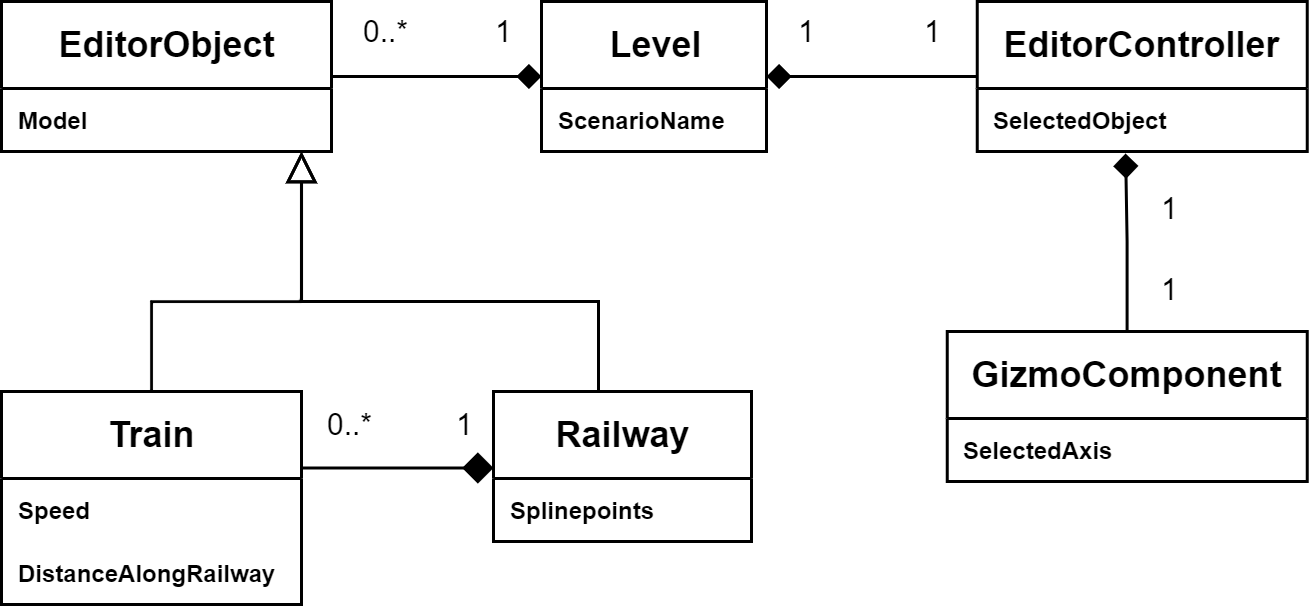
\includegraphics[width=0.9\textwidth]{figures/EditorERDiagram.png}}
    \caption[size=small]{Class diagram for the editor mode}
\end{figure} 
\vspace*{1 cm} %Temporary fix for tables going into eachother

\subsubsection{Authentication}

User authentication is done using the existing solution in use at Lokførerskolen. Their system uses two endpoints, the first receives a username and password and returns a JWT (Json Web Token) on success. The JWT is then sent to the second endpoint, which returns a JSON UserObject which contains info such as ID, Username, Roles, etc. 

When the program is launched a login screen is presented to the user, where a username and password must be entered. The user must be authenticated in order to use the software. If an error occurs, such as invalid username or password, or an error with the server, an error message is shown to the user. Once the user is authenticated their info is stored for the duration of the session. The user-info is never stored to any file, which means the user needs to log in again when the program is started again. Because the username, password nor token is ever stored locally, they cannot be extracted from local files in order to obtain private credentials.


%The system for authenticating user credentials utilizes REST-technology over HTTPS (Hypertext Transfer Protocol Secure). The authentication is done by sending a POST-request to the client's API with a username and a password formatted as a JSON object.

\vspace*{1 cm} %Temporary fix for tables going into eachother
\begin{figure}[!htb]
    \centerline{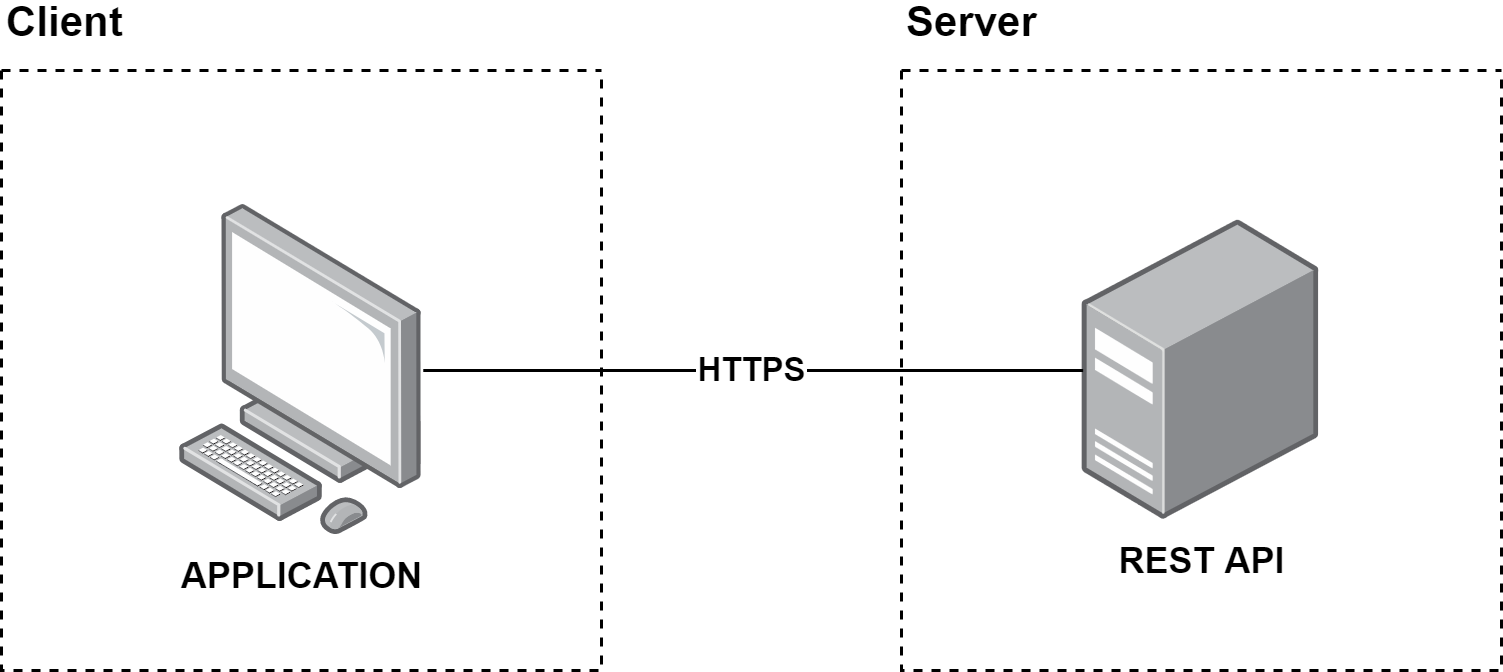
\includegraphics[width=0.9\textwidth]{figures/NetworkArchitecture.png}}
    \caption[size=small]{A diagram for the network architecture}
\end{figure} 

\subsubsection{Scenarios}
% System
\subsection{Design choices}
% 

% Have to figure out what to include in this section!
